\chapter{Teorija} \label{chapter:teorija} 

U ovom poglavlju se obrađuje teorija jezerskog skladišta podataka. Ne obrađuje
se cijela arhitektura nego samo odabrani slojevi te se daje definicija samog
jezerskog skladišta podataka. Odabrani slojevi su:
\begin{itemize}
    \item sloj unosa podataka,
    \item sloj pohrane podataka,
    \item sloj obrade podataka.
\end{itemize}
Odabirom određenih slojeva, u ovom radu se obrađuje samo dio arhitekture
jezerskog skladišta podataka, ali se obrađuje teorija koja je potrebna za
razumijevanje tehnologije koja se koristi u praktičnom dijelu rada. 

\section{Jezersko skladište podataka} \label{section:jezersko_skladiste_podataka}

Jezersko skladište podataka je arhitektura skladištenja
podataka koja kombinira karakteristike jezera podataka (eng. Data Lake) i
skladišta podataka (eng. Data Warehouse). To je centralizirano skladište
podataka koje omogućava analizu velike količine strukturiranih i
nestrukturiranih vrsta podataka u realnom vremenu ili u kasnijem trenutku.
jezersko skladište podataka omogućuje integraciju podataka iz različitih izvora,
olakšava upravljanje podacima, smanjuje troškove i vrijeme potrebno za pripremu
podataka za analizu. Ova arhitektura skladištenja podataka postaje sve
popularnija u posljednje vrijeme jer olakšava analizu podataka, izvještavanje i
donošenje odluka u stvarnom vremenu. Za detaljniji opis jezerskog skladišta
podataka vidjeti \cite{datalakehouse2022}.

\section{Sloj unosa podataka} \label{section:sloj_unosa_podataka}

Sloj unosa podataka (engl. Data Ingestion Layer) u jezerskom skladištu podataka
je sloj koji se koristi za prikupljanje i spremanje podataka iz različitih
izvora u jezersko skladište podataka. Ovaj sloj obuhvaća dva načina prikupljanja
podataka:
\begin{enumerate}
    \item serijsko prikupljanje podataka,
    \item strujno prikupljanje podataka.
\end{enumerate}

Sloj unosa podataka omogućuje podatkovnim inženjerima da učinkovito prikupe
podatke iz različitih izvora i formata, poput baza podataka, datoteka ili
senzorskih uređaja, te ih jednostavno učitaju u jezersko skladište podataka.
Ovaj sloj obično uključuje alate za obradu velikih količina podataka, poput
Apache Spark-a, kako bi se omogućilo brzo i učinkovito prikupljanje i spremanje
velikih količina podataka. Za detaljni opis sloja unosa podataka vidjeti
\cite{datalakehouse2022}.

\section{Sloj pohrane podataka} \label{section:sloj_pohrane_podataka}

U jezerskom skladištu podataka, sloj pohrane podataka obuhvaća skup tehnologija
i alata za pohranu velikih količina podataka u različitim formatima, kao što su
Apache Hadoop Distributed File System (HDFS), Amazon S3, Azure Blob Storage i
Google Cloud Storage.

Osim toga, Delta Lake tehnologija može se koristiti kao sloj pohrane podataka u
jezerskom skladištu, jer omogućuje verzioniranje podataka, upravljanje
transakcijama i omogućuje pohranu podataka u strukturiranom obliku, čime se
olakšava proces analize.

Podaci u sloju pohrane podataka se dijele na tri razine:
\begin{itemize}
    \item \textbf{sirovi podaci / brončani sloj} - podaci koji su prikupljeni iz izvora podataka,
    \item \textbf{obrađeni podaci / Srebrni sloj} - podaci koji su transformirani i pripremljeni za analizu,
    \item \textbf{analizirani podaci / zlatni sloj} - podaci koji su analizirani i spremljeni u agregiranom obliku.
\end{itemize}

Sloj pohrane podataka u jezerskom skladištu podataka mora biti oblikovan i
konfiguriran na način koji omogućuje brzi i jednostavan pristup podacima za
analizu, uz osiguravanje pouzdanosti, sigurnosti i skalabilnosti skladišta. Za
detaljni opis sloja pohrane podataka vidjeti \cite{datalakehouse2022}.

\section{Sloj obrade podataka} \label{section:sloj_obrade_podataka} 

Sloj obrade podataka (eng. Data Processing Layer) u jezerskom skladištu podataka
odnosi se na skup tehnologija i alata koji omogućuju obradu velikih količina
podataka pohranjenih u jezerskom skladištu podataka. Ovaj sloj obično uključuje
distribuirane obradne okvire, poput Apache Sparka, Apache Flinka i Apache Beama.

Sloj obrade podataka je dizajniran kako bi omogućio izvođenje različitih
operacija na podacima, uključujući čišćenje, transformiranje, spajanje i
agregiranje. Ovaj sloj omogućuje korisnicima da lako i učinkovito izvode složenu
obradu velikih skupova podataka, koristeći alate za distribuiranu obradu.

Sloj obrade podataka u jezerskom skladištu podataka igra ključnu ulogu u
omogućavanju pouzdane, skalabilne i brze obrade podataka pohranjenih u jezerskom
skladištu podataka, što omogućuje korisnicima da izvuku vrijednost iz podataka i
donose informirane poslovne odluke. Za detaljni opis sloja obrade podataka
vidjeti \cite{datalakehouse2022}.

\section{Arhitektura i tok podataka} \label{section:arhitektura_i_tok_podataka}

Arhitektura jezerskog skladišta podataka prikazana je na
slici~(\ref{figure:datalakehouse_architecture}). Ona proizlazi iz slojeva
opisanih u
poglavljima~(\ref{section:sloj_unosa_podataka}),~(\ref{section:sloj_pohrane_podataka})
i~(\ref{section:sloj_obrade_podataka}). Sloj unosa podataka samo upisuje podatke
u sloj pohrane pohrane podataka, dok sloj obrade podataka čita i piše podatke u
sloj pohrane podataka. Sloj obrade podataka čita i piše podatke jer u tom sloju
čišćenjem, transformiranjem, spajanjem i agregiranje podataka ostvaruju
podslojevi (brončani, srebrni i zlatni sloj) sloja pohrane podataka.

\begin{figure}[htb]
    \centering
    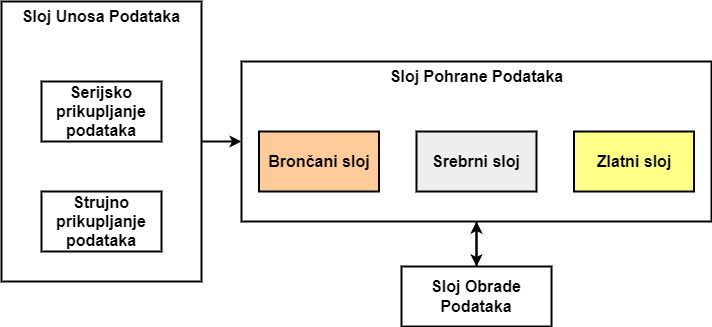
\includegraphics[width=0.8\textwidth]{images/arhitektura.drawio.png}
    \caption{Arhitektura modela jezerskog skladišta podataka.}
    \label{figure:datalakehouse_architecture}
\end{figure}

Sa slike~(\ref{figure:datalakehouse_data_flow}) se vidi da postoji tok podataka
između slojeva unosa, pohrane i obrade podataka. Sloj unosa podataka upisuje
podatke iz vanjske okoline (baze podataka, SFTP serveri, jezera podataka) u sloj
pohrane podataka. Unosom podataka se dobivaju sirovi podaci koje sloj obrade
podataka dohvaća i unosi u brončani sloj s najmanjim mogućim brojem
transformacija. Sljedeće, sloj obrade podataka dohvaća podatke iz brončanog
sloja te ih čisti, transformira i spaja. Obrađeni podaci brončanog sloja se
unose u srebrni sloj. Na kraju, sloj obrade podataka dohvaća podatke iz srebrnog
sloja te ih agregira i unosi u zlatni sloj. 

\begin{figure}
    \centering
    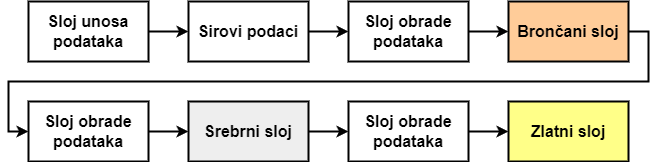
\includegraphics[width=0.8\textwidth]{images/tok_podataka.drawio.png}
    \caption{Tok podataka u jezerskom skladištu podataka.}
    \label{figure:datalakehouse_data_flow}
\end{figure}